\documentclass[12pt, paper=a4]{article}
\usepackage[utf8]{inputenc}
\usepackage[german]{babel}
\usepackage{mathrsfs}
\usepackage{amsmath}
\usepackage{amssymb}
\usepackage{listings}
\usepackage{graphicx}
\usepackage{fancyhdr}

\setlength{\parindent}{0pt}

\author{Mareike G\"ottsch, 6695217, Gruppe 2\\Paul H\"olzen, 6673477, Gruppe 1\\Sven Schmidt, 6217064, Gruppe 1}

\title{FGI 2 Hausaufgaben 11}

\rhead{M. G\"ottsch, G-2; P. H\"olzen, G-1; S. Schmidt, G-1}
\pagestyle{fancy}
\begin{document}
\maketitle

\section*{Aufgabe 11.3}
\subsection*{1.}
P/T-Netz siehe Abbildung 1.\\

\begin{figure}[h!]
\centering
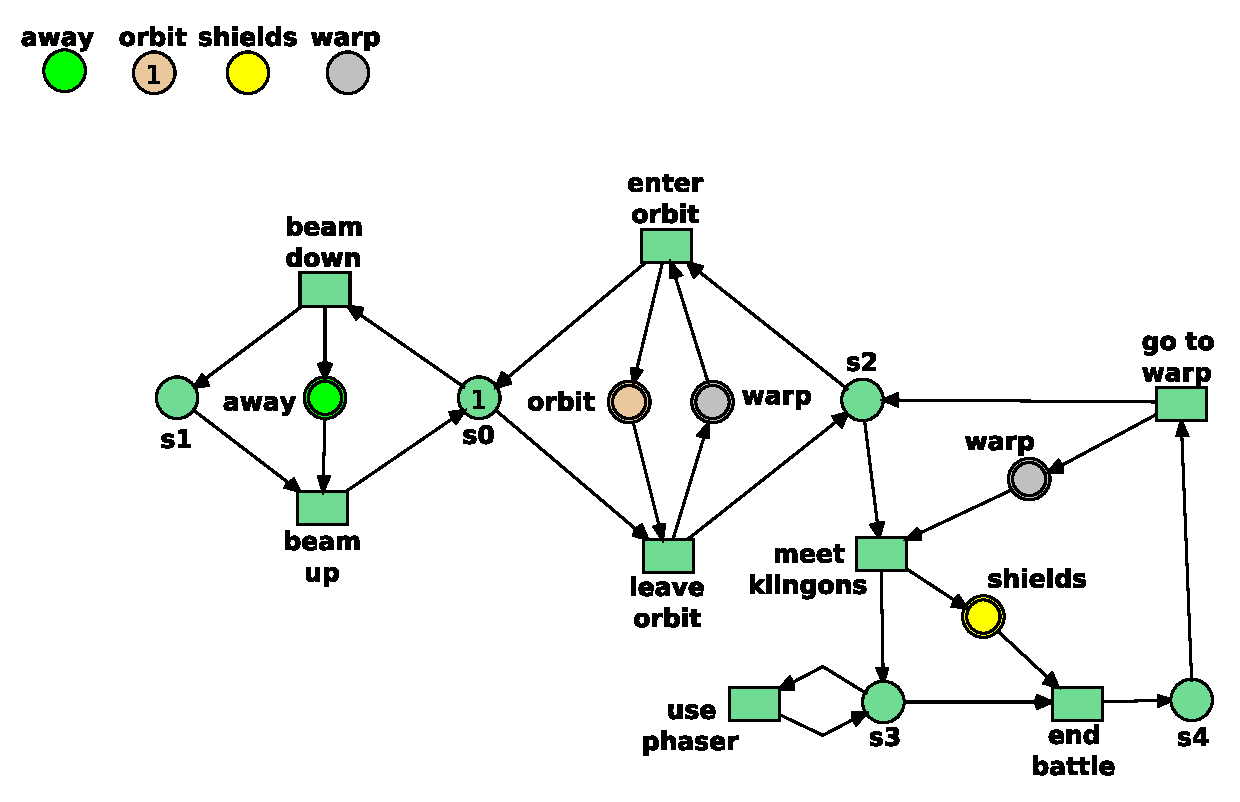
\includegraphics[scale=0.7]{EnterprisePT.pdf}
\caption{PT-Netz mit virtuellen Plätzen zum $TS_{Enterprise}$ aus Aufgabe 5.3}
\end{figure}

\subsection*{2.}
Formel: $f = AF(\not(orbit \Rightarrow away) \land \not AG(E(orbit U warp)))$\\
Lola-Syntax: \texttt{FORMULA ALLPATH EVENTUALLY (NOT (NOT orbit > 0 OR away > 0)) AND NOT ALLPATH ALWAYS (EXPATH [ orbit > 0 UNTIL warp > 0 ])}\\
Ergebnis: true\\

Formel: $g_1 = AGEF(warp)$\\
Lola-Syntax: \texttt{FORMULA ALLPATH ALWAYS EXPATH EVENTUALLY warp > 0}\\
Ergebnis: true\\

Formel: $g_2 = EFAG(warp)$\\
Lola-Syntax: \texttt{FORMULA EXPATH EVENTUALLY ALLPATH ALWAYS warp > 0}\\
Ergebnis: false\\

\subsection*{3.}
Formel: $AF(orbit \land EX(away))$\\
Lola-Syntax: \texttt{FORMULA ALLPATH EVENTUALLY (orbit > 0 AND EXPATH NEXTSTEP away > 0)}\\
Ergebnis: true\\
Sprachlich: Für alle Pfade, wenn irgendwann $orbit$ gilt, gibt es einen Pfad in dessen nächstem Schritt $away$ gilt.\\

Formel: $EF(shields)$\\
Lola-Syntax: \texttt{FORMULA EXPATH EVENTUALLY shields > 0}\\
Ergebnis: true\\
Sprachlich: Es gibt einen Pfad für den irgendwann mal $shields$ gilt.\\

Formel: $EF(warp \land shields)$\\
Lola-Syntax: \texttt{FORMULA EXPATH EVENTUALLY (warp > 0 AND shields > 0)}\\
Ergebnis: false\\
Sprachlich: Es gibt einen Pfad in dem irgendwann mal gleichzeitig $warp$ und $shields$ gelten.\\

Formel: $AF(away \land EX(warp))$\\
Lola-Syntax: \texttt{FORMULA ALLPATH EVENTUALLY (away > 0 AND EXPATH NEXTSTEP warp > 0)}\\
Ergebnis: false\\
Sprachlich: Für alle Pfade gilt irgendwann $away$ und es gibt dann einen Pfad in dessen nächsten Schritt $warp$ gilt.\\

\subsection*{4.}
In der Lola GUI in Renew wird eine Checkliste einiger statischer Netzeigenschaften angezeigt. Darunter auch Beschränktheit (Boundedness), Lebendigkeit (Liveness) und Reversibilität (Reversibility). Alle drei Eigenschaften werden vom Netz erfüllt.\\

\section*{Aufgabe 11.5}
\begin{itemize}
	\item Ein mehrfach gezeichneter Endzustand bezeichnet immer nur ein einziges Objekt. \\
		Wahr oder falsch?\\
		\textit{(Lesestoff Woche 11, Teil 1)}
	\item Der PAP-Kalk\"ul ist korrekt und vollst\"andig, d.h. \(s = t \Leftrightarrow s \overleftrightarrow{\underline{\quad}} t\).\\
		Wahr oder falsch?\\
		\textit{(Lesestoff Woche 11, Teil 1)}
\end{itemize}

\end{document}